\section{Synchronmaschine}
    \renewcommand{\arraystretch}{2.5}
{\scriptsize \textcolor{green}{Vorteil}:
\begin{itemize} 
	\item sehr robust, elektrodynamisch, mechanisch und thermisch stabil
    \item Hoher Wirkungsgrad (80-90\%)
	\item Drehmoment einfach bestimmbar
	\item Einfache Konstruktion
	\item Man kann Blindleistung mit diesem Motor kompensieren
\end{itemize}
\textcolor{red}{Nachteil}:
\begin{itemize}
\item Anlaufstrom
\end{itemize}}
\subsection{Funktionsweise}
Das Drehfeld und der Rotor einer Synchronmaschine rotieren mit derselben Geschwindigkeit d.h. sind sie im Synchronlauf. \\
\textbf{Anwendung:} zur Umwandlung von mechanischer Energie in elektrische Energie.
\subsection{Aufbau und Wirkungsprinzip}
    \begin{minipage}[b]{0.5\linewidth}
    	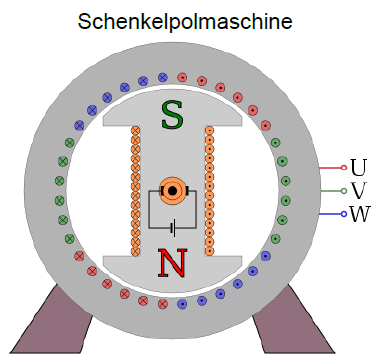
\includegraphics[width = 5cm]{images/Schenkelpolmaschine}
    \end{minipage}
    \begin{minipage}[b]{0.5\linewidth}
    	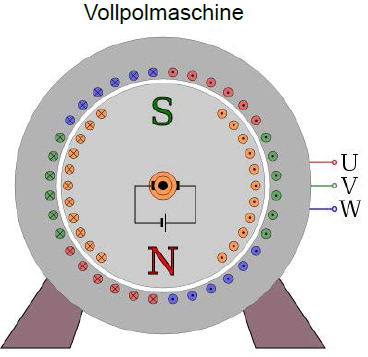
\includegraphics[width = 5cm]{images/Vollpolmaschine}
    \end{minipage}
    \begin{tabular}[b]{| C{0.4\linewidth} | C{0.4\linewidth} |}
    	\hline
    	\textbf{Schenkelpolmaschine} &
        \textbf{Vollpolmaschine}
        \\ \hline
        
    	\vspace{-0.7cm}
    	\begin{itemize}
    		\item Grössere Polpaarzahl
    		\item Kleinere Drehzahl
    		\item Wasserkraftwerk
    	\end{itemize} &
        \vspace{-0.7cm}
        \begin{itemize}
        	\item p = 1
        	\item Grössere Drehzahl
        	\item Wärmekraftwerke
        \end{itemize}
        \\ \hline
    \end{tabular}
    \\
    
    \begin{minipage}[b]{0.33\linewidth}
    	\raggedright
    	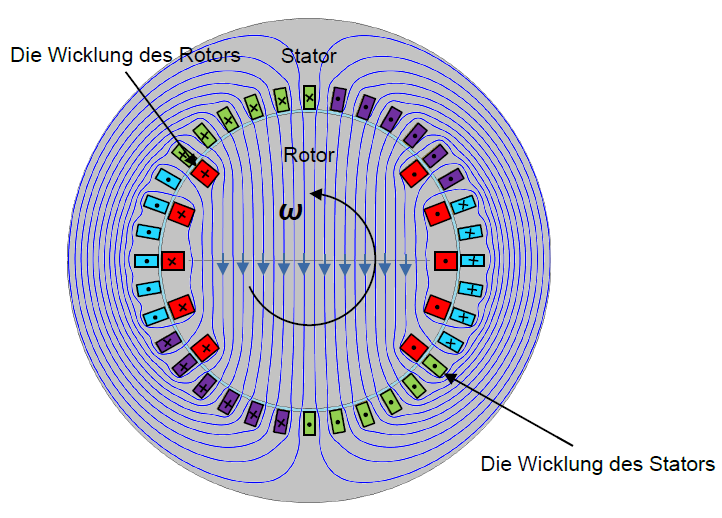
\includegraphics[width = 10cm]{images/AufbauSynchronmotor}
    \end{minipage}
    \clearpage
    \pagebreak

\subsection{Grundgleichungen}
    \begin{minipage}[b]{0.5\linewidth}
        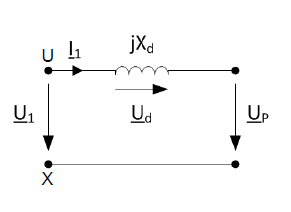
\includegraphics[width = 7cm]{images/Wicklung1}
    \end{minipage}
    \begin{minipage}[b]{0.5\linewidth}
        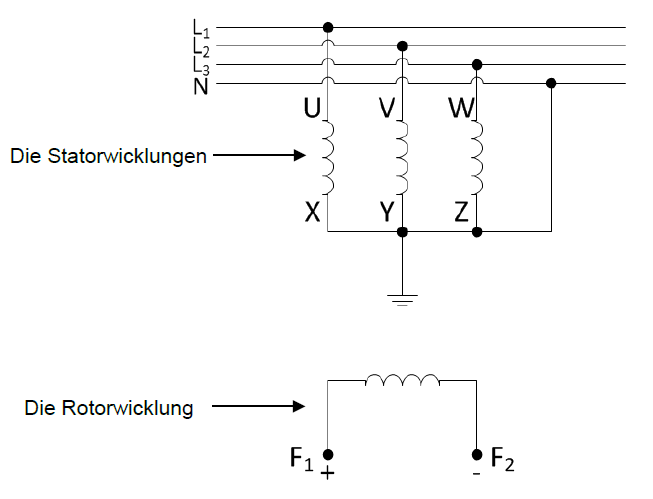
\includegraphics[width = 8cm]{images/Wicklungen}
    \end{minipage}
    \vspace{-1cm}
    \begin{tabular}[b]{| C{5cm}| P{8.5cm} | P{5 cm} |}
    	\hline
        \textbf{Strangspannung} 	&
        $\underline{U_1\!} = \underline{U_d\!} + \underline{U_P\!}$ &
        $U_P \, \widehat{=}$ der Polradspannung
        \\ \hline
        
        \textbf{Spulenspannung}	&
        $\underline{U_d} = jX_d\cdot \underline{I_1}$ &
        \\ \hline
        
        \textbf{Polradspannung} \newline (fiktive Hilfsgrösse) &
        $\underline{U_P} = \underline{U_P}\left(I_e\right)$ \newline\newline
        $\underline{U_P} = jX_h\cdot I_{e}\,'$  &
        $I_e \, \widehat{=}$ dem Erregerstrom \newline
        $I_e\,' \widehat{=}$ dem Erregerstrom umgerechnet auf die Statorseite
        \\ \hline
        
        \textbf{Synchronreaktanz} &
        $X_d = X_{\sigma 1} + X_h$ &
        $X_d \, \widehat{=} $ Synchronreaktanz \newline
        $X_{\sigma 1} \, \widehat{=}$ Streureaktanz des Stators \newline
        $X_h \, \widehat{=}$ der Hauptreaktanz
        \\ \hline
        
        \textbf{Leistung} \newline
        \tabbild[scale=0.4]{images/SynchronKennlinie} &
        $\varphi = -\alpha - \dfrac{\pi}{2}$ \newline
        $\cos(\varphi) = -\sin(\alpha)$ \newline
       	$ (X_d \cdot I_1)^2=(\frac{U_1}{\sqrt{3}})^2+(\frac{U_p}{\sqrt{3}})^2 - 2\cdot \frac{U_1}{\sqrt{3}}\cdot \frac{U_p}{\sqrt{3}} cos(\delta) $ \newline\newline
        \textbf{Generatorbetrieb:} $\delta < 0$ \newline
        \textcolor{red}{d} = $-U_p\cdot\sin(\delta)$ \newline
        \qquad $= X_d\cdot I_1\cdot\sin(\alpha) = -X_d\cdot I_1\cdot\cos(\varphi)$ \newline \newline
        $P(\delta) = 3\dfrac{U_P\cdot U_1}{X_d}\cdot\sin(\delta)$ \newline \newline
        $P(\delta) = P_{mech}-P_V = \omega\cdot M - P_V$ \newline \newline
        \textbf{Motorbetrieb:} $\delta > 0$ \newline
        $P(\delta) = P_{mech} + P_V = \omega\cdot M + P_V$ &
        Polradwinkel $\delta =  \measuredangle (U_p, U_1)$  \newline \newline
        $U_P$ ist die Polradspannung, sie entspricht einer fiktiven Grösse! Sie kann wiederum durch ein Zeigerdiagramm bestimmt werden.
        \\ \hline
		\textbf{Erreger-Regulierkennlinien} & 
		$ \dfrac{I_e}{I_{e0}} = \sqrt{cos^2(\varphi) + \left(x\cdot\dfrac{I_1}{I_N}-sin(\varphi)\right)^2}$ & $I_e = f(I_1)$ \newline $cos(\varphi)$ gegeben \newline $I_1$ - gewünschter Netzstrom \newline Bezugswert $x = \dfrac{X_d}{X_N}$
		\\ \hline
	    \end{tabular}
    \clearpage
    \newpage
    
    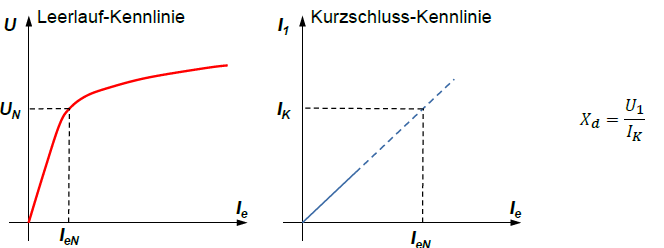
\includegraphics[scale = 0.8]{images/KennlinieSynchronmaschine}

\subsection{Zeigerdiagramm im Motorbetrieb}
    P > 0 und $\delta$ > 0 \newline \newline
    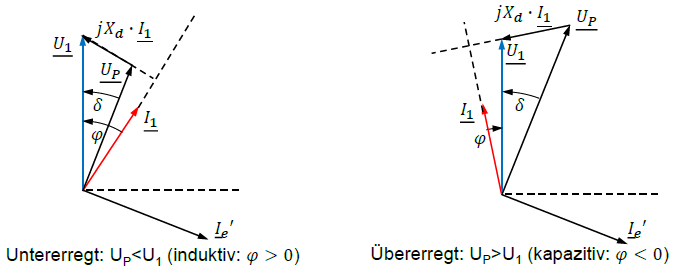
\includegraphics[width = 12 cm]{images/ZeigerdiagrammSynchronmaschine}

\subsection{Zeigerdiagramm im Generatorbetrieb}
    P < 0, $\delta$ < 0  \newline
    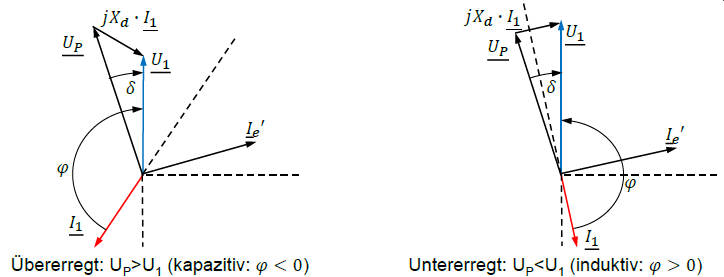
\includegraphics[width = 12 cm]{images/ZeigerdiagrammGeneratorbetrieb} \newline \newline
    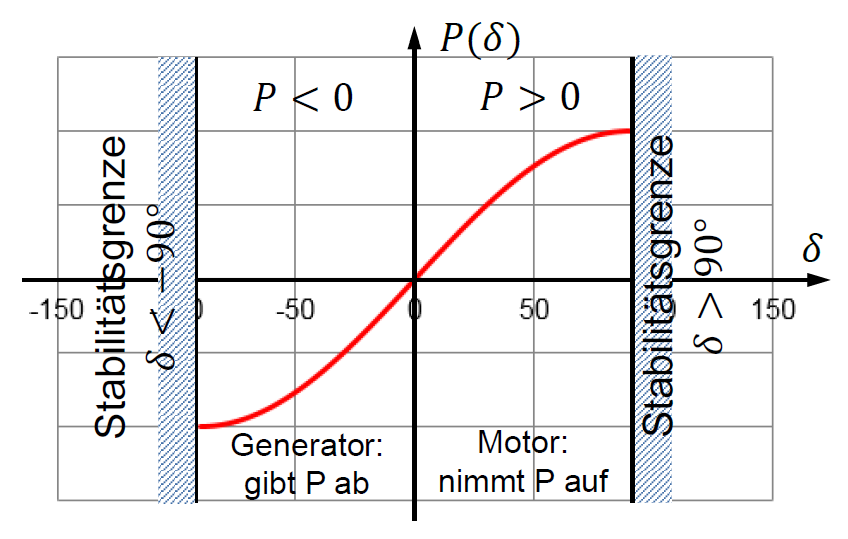
\includegraphics[scale = 0.4]{images/Stabilitaet}



\clearpage
\pagebreak
